% Simplex-Splat: Runtime Verification of Online 3DGS Mapping
% IEEE Conference Template for AA228V/CS238V Final Project
\documentclass[conference]{IEEEtran}

% ============================================================
% Packages
% ============================================================
\usepackage[utf8]{inputenc}
\usepackage[T1]{fontenc}
\usepackage{amsmath,amssymb,amsfonts}
\usepackage{algorithmic}
\usepackage{algorithm}
\usepackage{graphicx}
\usepackage{textcomp}
\usepackage{xcolor}
\usepackage{booktabs}
\usepackage{multirow}
\usepackage{hyperref}
\usepackage{subcaption}
\usepackage{pgfplots}
\usepackage{tikz}
\usetikzlibrary{shapes,arrows.meta,positioning,fit,backgrounds,calc,decorations.pathreplacing}
\pgfplotsset{compat=1.18}
\usepackage[style=ieee,backend=biber]{biblatex}
\addbibresource{references.bib}

% Color definitions for figures
\definecolor{tealaccent}{HTML}{20808D}
\definecolor{terracotta}{HTML}{A84B2F}
\definecolor{darkteal}{HTML}{1B474D}
\definecolor{lightcyan}{HTML}{BCE2E7}
\definecolor{mauvecol}{HTML}{944454}
\definecolor{goldcol}{HTML}{FFC553}
\definecolor{safezone}{HTML}{2E8B57}
\definecolor{dangerzone}{HTML}{C0392B}

% Placeholder command for values to be filled in
\newcommand{\placeholder}[1]{\textcolor{tealaccent}{\textbf{[#1]}}}

\begin{document}

\title{Simplex-Splat: Runtime Verification of Online 3D Gaussian Splatting Maps for Safe Autonomous Navigation}

\author{
\IEEEauthorblockN{Rahul Ayanampudi}
\IEEEauthorblockA{
Department of Aeronautics \& Astronautics\\
Stanford University\\
\texttt{rayanam@stanford.edu}}
\and
\IEEEauthorblockN{Carlo Schreiber}
\IEEEauthorblockA{
Department of Electrical Engineering\\
Stanford University\\
\texttt{carlops@stanford.edu}}
}

\maketitle

% ============================================================
% ABSTRACT
% ============================================================
\begin{abstract}
Neural radiance representations such as 3D Gaussian Splatting (3DGS) offer unprecedented visual fidelity for dense mapping in robotic systems, yet they provide no formal guarantees of geometric or semantic correctness---a critical gap for safety-critical autonomous navigation. We present \textsc{Simplex-Splat}, a runtime monitoring framework grounded in the Simplex Architecture that continuously validates an online 3DGS map against raw sensor streams. Our system implements a semantically-aware residual monitor that cross-references depth renders from the neural map with LiDAR-equivalent ground truth and semantic segmentation, triggering deterministic emergency braking when the map diverges from reality. We evaluate \textsc{Simplex-Splat} in the CARLA simulator across two adversarial scenarios---unmodeled dynamic pedestrians and unconverged static geometry---and compare a pure geometric monitor baseline against our semantically-aware variant. The semantically-aware monitor achieves a true positive rate of \placeholder{XX}\% with a false positive rate of \placeholder{XX}\% in static environments, while maintaining a safety response time of \placeholder{XX}\,ms, compared to the pure geometric baseline's false positive rate of \placeholder{XX}\%. An ablation study over residual threshold $\tau$ reveals the critical role of semantic filtering in achieving robust runtime verification without excessive conservatism.
\end{abstract}

\begin{IEEEkeywords}
Runtime verification, 3D Gaussian Splatting, Simplex Architecture, autonomous navigation, safety monitoring
\end{IEEEkeywords}

% ============================================================
% I. INTRODUCTION
% ============================================================
\section{Introduction}
\label{sec:intro}

The adoption of neural scene representations for dense mapping in robotics has accelerated rapidly. 3D Gaussian Splatting (3DGS)~\cite{kerbl2023gaussian} has emerged as a compelling alternative to Neural Radiance Fields (NeRFs)~\cite{mildenhall2020nerf} by representing scenes as collections of anisotropic 3D Gaussians that can be rendered in real time via differentiable rasterization. Recent works such as SplaTAM~\cite{keetha2024splatam} demonstrate that 3DGS can be integrated into online Simultaneous Localization and Mapping (SLAM) pipelines, achieving sub-centimeter tracking accuracy and photorealistic reconstruction at 400\,FPS.

However, the use of these probabilistic representations in safety-critical autonomy introduces significant risks. Unlike classical geometric maps built from LiDAR point clouds, 3DGS maps are optimized via gradient descent and are susceptible to failure modes that are fundamentally different from traditional mapping artifacts:

\begin{itemize}
    \item \textbf{Phantom obstacles:} Unconverged Gaussians can hallucinate geometry in free space, causing unnecessary emergency stops.
    \item \textbf{Ghost artifacts:} Dynamic actors (e.g., pedestrians) that move away leave residual Gaussians in the map, producing stale occupancy estimates.
    \item \textbf{Missing geometry:} Newly appeared objects may not yet be reconstructed by the online optimization, creating blind spots in the planner's world model.
\end{itemize}

A planner that trusts a 3DGS map without verification risks both \emph{phantom braking} (false positive safety interventions due to artifacts) and \emph{missed detections} (false negative failures where real obstacles are absent from the map). These failure modes are especially dangerous in urban environments with dynamic, unpredictable actors.

To address this gap, we propose \textsc{Simplex-Splat}, a runtime monitoring framework based on the Simplex Architecture~\cite{sha2001simplex}. The Simplex Architecture is a well-established paradigm for runtime assurance in which a high-assurance decision module monitors the output of an unverified advanced controller and switches to a verified baseline controller when safety violations are imminent~\cite{bak2014simplex, desai2019soter}. We adapt this principle from the \emph{control} domain to the \emph{perception} domain: instead of monitoring controller commands, our decision module monitors the \emph{map} itself by cross-validating neural renders against raw sensor streams.

Our contributions are as follows:
\begin{enumerate}
    \item A runtime verification framework (\textsc{Simplex-Splat}) that adapts the Simplex Architecture to validate online 3DGS maps against ground-truth sensors.
    \item A semantically-aware residual monitor that restricts depth validation to safety-critical object classes, significantly reducing false positive rates compared to a pure geometric baseline.
    \item A formal safety specification $\phi_{\text{safe}}$ encompassing dynamic safety, static integrity, and structural consistency.
    \item Quantitative evaluation in the CARLA simulator across adversarial scenarios with ablation studies over monitoring parameters.
\end{enumerate}

% ============================================================
% II. RELATED WORK
% ============================================================
\section{Related Work}
\label{sec:related}

\subsection{3D Gaussian Splatting for Dense Mapping}

3D Gaussian Splatting~\cite{kerbl2023gaussian} represents scenes as a set of 3D Gaussians, each parameterized by a mean $\boldsymbol{\mu} \in \mathbb{R}^3$, covariance $\boldsymbol{\Sigma} \in \mathbb{R}^{3\times3}$, opacity $\alpha \in [0,1]$, and view-dependent color encoded via spherical harmonics. Rendering is performed by projecting Gaussians onto the image plane and alpha-compositing in depth order, enabling real-time frame rates on commodity GPUs.

SplaTAM~\cite{keetha2024splatam} extends 3DGS to online dense SLAM from an unposed RGB-D camera. It introduces silhouette-guided tracking, where the rendered opacity mask guides camera pose optimization via differentiable rendering. SplaTAM achieves up to $2\times$ improvement over prior dense SLAM methods~\cite{sucar2021imap, zhu2022nice, sandstrom2023pointslam} on camera pose estimation. In the autonomous driving domain, SplatAD~\cite{hess2024splatad} extends 3DGS to jointly render camera and LiDAR data with sensor-specific phenomena such as rolling shutter and ray dropout, achieving state-of-the-art rendering quality.

While these methods advance the fidelity and speed of neural mapping, none provide formal guarantees about the geometric correctness of their output---a prerequisite for deployment in safety-critical applications.

\subsection{The Simplex Architecture and Runtime Assurance}

The Simplex Architecture, introduced by Sha~\cite{sha2001simplex}, provides a framework for using complex, unverified controllers alongside simple, verified baseline controllers. The core idea is a \emph{decision module} that monitors system state and switches from the advanced to the baseline controller when the system approaches the boundary of a safe operating region.

Bak et al.~\cite{bak2014simplex} formalize the ``Black-Box Simplex Architecture,'' removing the requirement for verified baseline controllers by instead relying on runtime checks of the baseline's output. Phan et al.~\cite{phan2023neural} demonstrate neural reachability-based runtime assurance for autonomous vehicles, using neural networks to approximate reachable sets within a Simplex framework. Desai et al.~\cite{desai2019soter} present SOTER, a language-based RTA framework for distributed robotic systems on ROS.

These works focus on \emph{control-level} assurance---monitoring controller commands and vehicle dynamics. Our work extends the Simplex paradigm to the \emph{perception level}, monitoring the neural map representation itself.

\subsection{Runtime Monitoring of Neural Representations}

The intersection of runtime verification and neural scene representations remains largely unexplored. PreSight~\cite{yuan2024presight} uses city-scale NeRF priors to enhance online perception but does not provide safety monitoring. Autonomous driving benchmarks in CARLA~\cite{dosovitskiy2017carla} evaluate perception and planning pipelines end-to-end but lack dedicated map-level validation.

To our knowledge, \textsc{Simplex-Splat} is the first framework to apply runtime verification principles to online 3DGS maps, providing a principled mechanism for detecting and mitigating neural map failures during autonomous navigation.

% ============================================================
% III. PROBLEM FORMULATION
% ============================================================
\section{Problem Formulation}
\label{sec:problem}

\subsection{Setting}

Consider an autonomous agent navigating an urban environment. At each discrete time step $k$, the agent receives an RGB-D observation $\mathbf{o}_k = (\mathbf{I}_k^{\text{rgb}}, \mathbf{D}_k^{\text{obs}})$ and its ground-truth pose $\mathbf{T}_k \in SE(3)$. The agent maintains an online 3DGS map $\mathcal{M}_k$ via a modified SplaTAM pipeline, which it uses for downstream path planning.

We assume access to a ground-truth sensor suite providing:
\begin{itemize}
    \item LiDAR-equivalent depth: $\mathbf{D}_k^{\text{obs}} \in \mathbb{R}^{H \times W}$
    \item Semantic segmentation: $\mathbf{S}_k^{\text{obs}} \in \mathcal{C}^{H \times W}$, where $\mathcal{C} = \{\text{Vehicle}, \text{Pedestrian}, \text{StopSign}, \text{Drivable}, \ldots\}$
\end{itemize}

This assumption isolates mapping errors from sensor noise and state estimation drift, allowing rigorous evaluation of the monitor's ability to detect neural map failures.

\subsection{Safety Specification}

We define a safety specification $\phi_{\text{safe}}$ as the conjunction of three properties that must hold at every time step:

\paragraph{Dynamic Safety ($\phi_{\text{dyn}}$)}
Any safety-critical dynamic object (Pedestrian, Vehicle) detected by the semantic sensor must have a corresponding presence in the neural map. Formally, for every pixel $(i,j)$ where $\mathbf{S}_k^{\text{obs}}(i,j) \in \{\text{Ped}, \text{Veh}\}$:
\begin{equation}
    \label{eq:dyn_safety}
    |\mathbf{D}_k^{\text{pred}}(i,j) - \mathbf{D}_k^{\text{obs}}(i,j)| < \tau_{\text{fn}}
\end{equation}
where $\mathbf{D}_k^{\text{pred}}$ is the depth rendered from the 3DGS map at pose $\mathbf{T}_k$. A violation implies the map predicts empty space where a real obstacle exists.

\paragraph{Static Integrity ($\phi_{\text{static}}$)}
The map's predicted depth in drivable regions must not \emph{underestimate} observed free space beyond a safety margin:
\begin{equation}
    \label{eq:static_integrity}
    \forall (i,j) \text{ s.t. } \mathbf{S}_k^{\text{obs}}(i,j) = \text{Drivable}: \quad \mathbf{D}_k^{\text{pred}}(i,j) \geq \mathbf{D}_k^{\text{obs}}(i,j) - \tau_{\text{fp}}
\end{equation}
A violation indicates phantom geometry hallucinated by the neural map in drivable space.

\paragraph{Structural Consistency ($\phi_{\text{struct}}$)}
Critical static features (e.g., Stop Signs) must maintain structural consistency between the rendered map and ground truth, measured by Intersection over Union:
\begin{equation}
    \label{eq:struct}
    \text{IoU}(\mathbf{S}_k^{\text{pred}}, \mathbf{S}_k^{\text{obs}}, c) \geq \tau_{\text{IoU}} \quad \forall c \in \mathcal{C}_{\text{critical}}
\end{equation}

The overall safety specification is $\phi_{\text{safe}} = \phi_{\text{dyn}} \wedge \phi_{\text{static}} \wedge \phi_{\text{struct}}$.

% ============================================================
% IV. APPROACH
% ============================================================
\section{Approach: The \textsc{Simplex-Splat} Architecture}
\label{sec:approach}

\subsection{System Overview}

\textsc{Simplex-Splat} implements a Simplex Architecture with three components, illustrated in Fig.~\ref{fig:system_arch}:

\begin{enumerate}
    \item \textbf{Advanced Channel (AC):} The online 3DGS map $\mathcal{M}_k$ built by a modified SplaTAM pipeline within a sliding window of $\sim$50\,m. The path planner queries this map for obstacle-free trajectories.
    \item \textbf{Safety Monitor (DM):} A high-assurance decision module that, at every time step, renders the expected depth $\mathbf{D}_k^{\text{pred}}$ and semantic view $\mathbf{S}_k^{\text{pred}}$ from the vehicle's pose and computes a hybrid residual against the ground-truth sensor stream.
    \item \textbf{Baseline Controller (BC):} A deterministic emergency braking controller that decelerates the vehicle to a full stop when the monitor triggers a safety violation.
\end{enumerate}

\begin{figure*}[!t]
    \centering
    % System Architecture: Simplex-Track
% Three clear sections left-to-right: Advanced Channel → Decision Module → Actuation
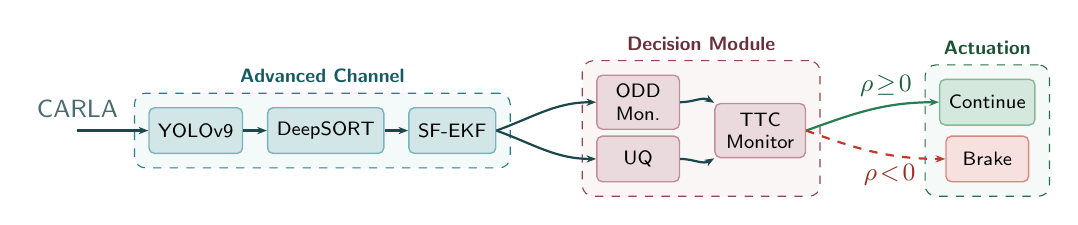
\begin{tikzpicture}[
    node distance=0.30cm and 0.30cm,
    block/.style={rectangle, draw, minimum height=0.58cm, minimum width=1.05cm,
                  align=center, font=\scriptsize\sffamily, rounded corners=2pt, line width=0.5pt},
    advanced/.style={block, fill=tealaccent!20, draw=tealaccent!60},
    monitor/.style={block, fill=mauvecol!20,    draw=mauvecol!60},
    baseline/.style={block, fill=dangerzone!15, draw=dangerzone!60},
    output/.style={block, fill=safezone!20,     draw=safezone!60},
    arrow/.style={-{Stealth[length=3.5pt]}, thick, color=darkteal},
    dasharrow/.style={-{Stealth[length=3.5pt]}, thick, dashed, color=dangerzone},
    lbl/.style={font=\small\sffamily\bfseries},
    grouplabel/.style={font=\scriptsize\sffamily\bfseries},
]

% ── Advanced Channel (left section) ─────────────────────────────────────────
\node[advanced] (yolo)     {YOLOv9};
\node[advanced, right=of yolo]     (deepsort) {DeepSORT};
\node[advanced, right=of deepsort] (sfekf)    {SF-EKF};

% ── Decision Module (middle section) ─────────────────────────────────────────
% ODD and UQ stacked to the left of TTC, all inside the Decision Module box
\coordinate (dmLeft) at ($(sfekf.east)+(1.8cm, 0)$);
\node[monitor, minimum width=1.05cm] (odd) at ($(dmLeft)+(0, 0.36cm)$)  {ODD\\Mon.};
\node[monitor, minimum width=1.05cm] (uq)  at ($(dmLeft)+(0,-0.36cm)$)  {UQ};
\node[monitor, minimum width=1.15cm] (ttc) at ($(dmLeft)+(1.55cm, 0)$)  {TTC\\Monitor};

% ── Actuation (right section) ─────────────────────────────────────────────
\node[output,   minimum width=1.05cm] (cont)  at ($(ttc.east)+(2.3cm, 0.36cm)$)  {Continue};
\node[baseline, minimum width=1.05cm] (estop) at ($(ttc.east)+(2.3cm,-0.36cm)$)  {Brake};

% ── Advanced Channel pipeline ─────────────────────────────────────────────
\draw[arrow] ([xshift=-0.90cm]yolo.west) -- (yolo.west);
\node[above=0.04cm, font=\small\sffamily, color=darkteal!80, align=center]
    at ([xshift=-0.90cm]yolo.west) {CARLA};
\draw[arrow] (yolo)     -- (deepsort);
\draw[arrow] (deepsort) -- (sfekf);

% ── SF-EKF fans into ODD and UQ ──────────────────────────────────────────
\draw[arrow] (sfekf.east) to[out=20,  in=180] (odd.west);
\draw[arrow] (sfekf.east) to[out=-20, in=180] (uq.west);

% ── ODD and UQ feed into TTC ──────────────────────────────────────────────
\draw[arrow] (odd.east) to[out=0, in=150] (ttc.north west);
\draw[arrow] (uq.east)  to[out=0, in=210] (ttc.south west);

% ── TTC decision outputs with clear ρ labels ──────────────────────────────
\draw[arrow, color=safezone!80!darkteal]
    (ttc.east) to[out=20, in=180] (cont.west);
\draw[dasharrow]
    (ttc.east) to[out=-20, in=180] (estop.west);
% ρ labels placed explicitly at 60% of the way into the gap
\node[lbl, color=safezone!70!black]
    at ($(ttc.east)!0.60!(cont.west)+(0,0.35cm)$)  {$\rho\!\geq\!0$};
\node[lbl, color=dangerzone!80!black]
    at ($(ttc.east)!0.60!(estop.west)+(0,-0.35cm)$) {$\rho\!<\!0$};

% ── Group bounding boxes (on background) ─────────────────────────────────
\begin{scope}[on background layer]
    \node[draw=tealaccent, dashed, fill=tealaccent!5, rounded corners=4pt,
          fit=(yolo)(deepsort)(sfekf), inner sep=5pt,
          label={[grouplabel, color=tealaccent!70!black, anchor=south]above:Advanced Channel}] {};
    \node[draw=mauvecol, dashed, fill=mauvecol!5, rounded corners=4pt,
          fit=(odd)(uq)(ttc), inner sep=5pt,
          label={[grouplabel, color=mauvecol!70!black, anchor=south]above:Decision Module}] {};
    \node[draw=safezone!80!black, dashed, fill=safezone!5, rounded corners=4pt,
          fit=(cont)(estop), inner sep=5pt,
          label={[grouplabel, color=safezone!60!black, anchor=south]above:Actuation}] {};
\end{scope}

\end{tikzpicture}

    \caption{The \textsc{Simplex-Splat} architecture. The Advanced Channel (left) uses a SplaTAM-based 3DGS map for path planning. The Safety Monitor (center) cross-validates rendered depth/semantics against ground-truth sensors. Upon detecting a violation of $\phi_{\text{safe}}$, control is transferred to the Emergency Braking baseline controller (right).}
    \label{fig:system_arch}
\end{figure*}

\subsection{Semantically-Aware Residual Monitor}

The core of our safety monitor is a \emph{semantically-aware residual computation} that restricts depth validation to safety-critical regions, rather than computing global pixel-wise residuals.

At each time step $k$, the monitor:
\begin{enumerate}
    \item \textbf{Renders} the predicted depth $\mathbf{D}_k^{\text{pred}}$ and semantic map $\mathbf{S}_k^{\text{pred}}$ from the 3DGS map at the current pose $\mathbf{T}_k$.
    \item \textbf{Computes semantic masks} for safety-critical classes:
    \begin{equation}
        \mathbf{M}_c = \{(i,j) \mid \mathbf{S}_k^{\text{obs}}(i,j) = c\}, \quad c \in \mathcal{C}_{\text{critical}}
    \end{equation}
    \item \textbf{Evaluates masked residuals} for each specification component:
    \begin{align}
        r_{\text{dyn}} &= \frac{1}{|\mathbf{M}_{\text{dyn}}|} \sum_{(i,j) \in \mathbf{M}_{\text{dyn}}} \mathbb{1}\!\left[|\Delta D_{ij}| > \tau_{\text{fn}}\right] \label{eq:r_dyn} \\
        r_{\text{static}} &= \frac{1}{|\mathbf{M}_{\text{drv}}|} \sum_{(i,j) \in \mathbf{M}_{\text{drv}}} \mathbb{1}\!\left[\mathbf{D}_k^{\text{pred}}(i,j) < \mathbf{D}_k^{\text{obs}}(i,j) - \tau_{\text{fp}}\right] \label{eq:r_static}
    \end{align}
    where $\Delta D_{ij} = \mathbf{D}_k^{\text{pred}}(i,j) - \mathbf{D}_k^{\text{obs}}(i,j)$ and $\mathbf{M}_{\text{dyn}} = \mathbf{M}_{\text{Ped}} \cup \mathbf{M}_{\text{Veh}}$.
    \item \textbf{Triggers handover} to emergency braking if any residual exceeds its threshold:
    \begin{equation}
        \text{trigger} = (r_{\text{dyn}} > \epsilon_{\text{dyn}}) \lor (r_{\text{static}} > \epsilon_{\text{static}}) \lor (\text{IoU} < \tau_{\text{IoU}})
    \end{equation}
\end{enumerate}

This semantic filtering is critical: a purely geometric monitor that computes residuals globally (over all pixels) is susceptible to false alarms from depth noise in background regions, foliage, and sky boundaries. By restricting attention to safety-critical masks, we achieve robust monitoring without excessive conservatism.

The full monitoring procedure is summarized in Algorithm~\ref{alg:monitor}.

\begin{algorithm}[!t]
\caption{\textsc{Simplex-Splat} Safety Monitor}
\label{alg:monitor}
\begin{algorithmic}[1]
\REQUIRE Pose $\mathbf{T}_k$, 3DGS map $\mathcal{M}_k$, sensors $(\mathbf{D}_k^{\text{obs}}, \mathbf{S}_k^{\text{obs}})$
\REQUIRE Thresholds $\tau_{\text{fn}}, \tau_{\text{fp}}, \tau_{\text{IoU}}, \epsilon_{\text{dyn}}, \epsilon_{\text{static}}$
\ENSURE Action $\in \{\text{CONTINUE}, \text{E-STOP}\}$
\STATE Render $\mathbf{D}_k^{\text{pred}}, \mathbf{S}_k^{\text{pred}} \leftarrow \textsc{Render}(\mathcal{M}_k, \mathbf{T}_k)$
\STATE $\mathbf{M}_{\text{dyn}} \leftarrow \{(i,j) \mid \mathbf{S}_k^{\text{obs}}(i,j) \in \{\text{Ped, Veh}\}\}$
\STATE $\mathbf{M}_{\text{drv}} \leftarrow \{(i,j) \mid \mathbf{S}_k^{\text{obs}}(i,j) = \text{Drivable}\}$
\STATE $r_{\text{dyn}} \leftarrow \frac{1}{|\mathbf{M}_{\text{dyn}}|} \sum_{(i,j) \in \mathbf{M}_{\text{dyn}}} \mathbb{1}[|\Delta D_{ij}| > \tau_{\text{fn}}]$
\STATE $r_{\text{static}} \leftarrow \frac{1}{|\mathbf{M}_{\text{drv}}|} \sum_{(i,j) \in \mathbf{M}_{\text{drv}}} \mathbb{1}[\mathbf{D}_k^{\text{pred}}(i,j) < \mathbf{D}_k^{\text{obs}}(i,j) - \tau_{\text{fp}}]$
\STATE $\textit{iou} \leftarrow \textsc{IoU}(\mathbf{S}_k^{\text{pred}}, \mathbf{S}_k^{\text{obs}}, \mathcal{C}_{\text{critical}})$
\IF{$r_{\text{dyn}} > \epsilon_{\text{dyn}}$ \textbf{or} $r_{\text{static}} > \epsilon_{\text{static}}$ \textbf{or} $\textit{iou} < \tau_{\text{IoU}}$}
    \RETURN \textsc{E-Stop}
\ELSE
    \RETURN \textsc{Continue}
\ENDIF
\end{algorithmic}
\end{algorithm}

\subsection{Sliding-Window Map Management}

To maintain bounded computational complexity, the 3DGS map is managed within a sliding window centered on the vehicle's current position. Gaussians beyond the window boundary ($\sim$50\,m) are pruned, ensuring $O(1)$ query complexity and constant memory usage. New Gaussians are added only in previously unmapped regions using SplaTAM's silhouette-guided densification strategy.

\subsection{Emergency Braking Controller}

The baseline controller implements maximum-deceleration braking with a simple kinematic model:
\begin{equation}
    a_{\text{brake}} = -a_{\max}, \quad v_{k+1} = \max(0, v_k + a_{\text{brake}} \cdot \Delta t)
\end{equation}
This controller is trivially verifiable and guaranteed to bring the vehicle to a stop within a bounded distance $d_{\text{stop}} = v_k^2 / (2 a_{\max})$.

% ============================================================
% V. EXPERIMENTAL SETUP
% ============================================================
\section{Experimental Setup}
\label{sec:experiments}

\subsection{Simulation Environment}

All experiments are conducted in CARLA~\cite{dosovitskiy2017carla} (v0.9.13+) operating in \emph{synchronous mode} with a fixed time step $\Delta t = 0.05$\,s (20\,Hz). This design choice decouples simulation time from wall-clock rendering time, ensuring that all validation metrics reflect the algorithmic performance of the monitor rather than hardware-dependent timing artifacts. We use Town10HD as the primary map, which provides a dense urban environment with varied road geometry, signage, and pedestrian infrastructure.

\subsection{Sensor Configuration}

The ego vehicle is equipped with:
\begin{itemize}
    \item \textbf{RGB Camera:} $1920 \times 1080$, 90$^\circ$ FoV, mounted at hood level.
    \item \textbf{Depth Sensor:} Ground-truth depth from CARLA's depth camera, providing $\mathbf{D}_k^{\text{obs}}$ at the same resolution.
    \item \textbf{Semantic Segmentation:} CARLA's ground-truth semantic camera, providing per-pixel class labels $\mathbf{S}_k^{\text{obs}}$.
\end{itemize}

We explicitly assume perfect localization (ground-truth pose from CARLA) to rigorously isolate mapping errors from state estimation drift.

\subsection{Adversarial Scenarios}

We design two adversarial scenarios to test distinct failure modes of the 3DGS map:

\paragraph{Scenario 1: ``The Ghost'' (Dynamic Safety)}
A pedestrian jaywalks across the vehicle's planned trajectory. The SplaTAM pipeline, operating on a keyframe-based update schedule, fails to reconstruct the pedestrian in real time. The monitor must detect the discrepancy between the map (which shows free space) and the depth sensor (which shows an obstacle) and trigger emergency braking. This scenario targets $\phi_{\text{dyn}}$.

\paragraph{Scenario 2: ``The Blind Map'' (Static Integrity)}
A large static obstacle (e.g., a construction barrier) or Stop Sign is placed at a location that the 3DGS map has not yet converged on, resulting in either missing geometry or phantom artifacts. This tests $\phi_{\text{static}}$ and $\phi_{\text{struct}}$ by requiring the monitor to detect unconverged or hallucinated map regions.

Each scenario is run for \placeholder{N} trials with randomized spawn positions and timing to compute aggregate statistics. Fig.~\ref{fig:scenarios} illustrates the two adversarial scenarios.

\begin{figure*}[!t]
    \centering
    % Scenario Overview Diagrams
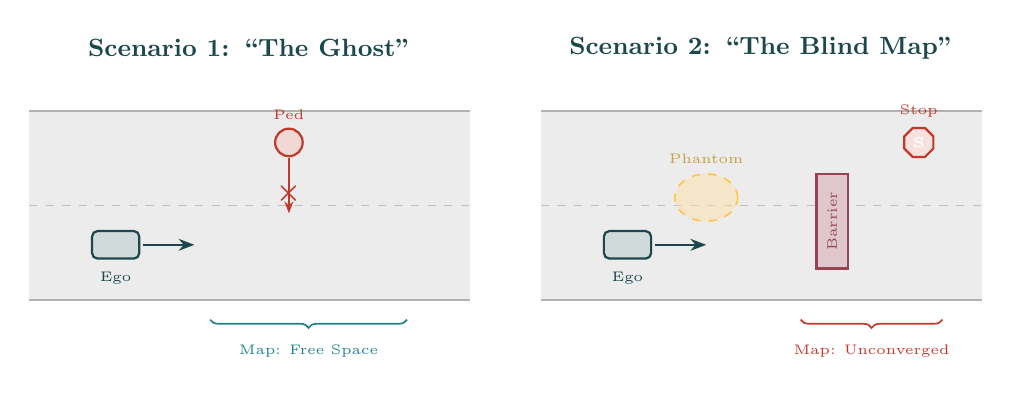
\begin{tikzpicture}[
    node distance=0.5cm,
    font=\small,
]

% ============================================================
% SCENARIO 1: THE GHOST
% ============================================================
\begin{scope}[shift={(0,0)}]
    % Road
    \fill[gray!15] (-0.3,-1.2) rectangle (5.3,1.2);
    \draw[gray!50, dashed, line width=0.5pt] (-0.3,0) -- (5.3,0);
    \draw[gray!60, line width=1pt] (-0.3,-1.2) -- (5.3,-1.2);
    \draw[gray!60, line width=1pt] (-0.3,1.2) -- (5.3,1.2);

    % Ego vehicle
    \node[draw=darkteal, fill=darkteal!20, rounded corners=2pt, minimum width=0.6cm, minimum height=0.35cm, line width=0.8pt] (ego1) at (0.8,-0.5) {};
    \node[font=\tiny, text=darkteal, below=1pt of ego1] {Ego};
    \draw[-{Stealth[length=2mm]}, darkteal, line width=0.8pt] (1.15,-0.5) -- (1.8,-0.5);

    % Pedestrian crossing
    \node[draw=dangerzone, fill=dangerzone!20, circle, minimum size=0.35cm, line width=0.8pt] (ped1) at (3.0,0.8) {};
    \draw[-{Stealth[length=1.5mm]}, dangerzone, line width=0.8pt] (3.0,0.6) -- (3.0,-0.1);
    \node[font=\tiny, text=dangerzone] at (3.0,1.15) {Ped};

    % Map view shows free space
    \draw[tealaccent, line width=0.6pt, decorate, decoration={brace, amplitude=3pt, mirror}] (2.0,-1.45) -- (4.5,-1.45);
    \node[font=\tiny, text=tealaccent] at (3.25,-1.85) {Map: Free Space};

    % Red X for discrepancy
    \node[font=\normalsize, text=dangerzone] at (3.0,0.15) {$\boldsymbol{\times}$};

    % Title
    \node[font=\small\bfseries, text=darkteal] at (2.5,2.0) {Scenario 1: ``The Ghost''};
\end{scope}

% ============================================================
% SCENARIO 2: THE BLIND MAP
% ============================================================
\begin{scope}[shift={(6.5,0)}]
    % Road
    \fill[gray!15] (-0.3,-1.2) rectangle (5.3,1.2);
    \draw[gray!50, dashed, line width=0.5pt] (-0.3,0) -- (5.3,0);
    \draw[gray!60, line width=1pt] (-0.3,-1.2) -- (5.3,-1.2);
    \draw[gray!60, line width=1pt] (-0.3,1.2) -- (5.3,1.2);

    % Ego vehicle
    \node[draw=darkteal, fill=darkteal!20, rounded corners=2pt, minimum width=0.6cm, minimum height=0.35cm, line width=0.8pt] (ego2) at (0.8,-0.5) {};
    \node[font=\tiny, text=darkteal, below=1pt of ego2] {Ego};
    \draw[-{Stealth[length=2mm]}, darkteal, line width=0.8pt] (1.15,-0.5) -- (1.8,-0.5);

    % Static obstacle (barrier)
    \fill[mauvecol!30] (3.2,-0.8) rectangle (3.6,0.4);
    \draw[mauvecol, line width=1pt] (3.2,-0.8) rectangle (3.6,0.4);
    \node[font=\tiny, text=mauvecol, rotate=90] at (3.4,-0.2) {Barrier};

    % Stop sign
    \node[draw=dangerzone, fill=dangerzone!15, regular polygon, regular polygon sides=8, minimum size=0.4cm, line width=0.8pt] (stop) at (4.5,0.8) {};
    \node[font=\tiny, text=white] at (4.5,0.8) {\textbf{S}};
    \node[font=\tiny, text=dangerzone] at (4.5,1.2) {Stop};

    % Ghost artifact in map
    \fill[goldcol!50, opacity=0.5] (1.8,0.1) ellipse (0.4 and 0.3);
    \draw[goldcol, dashed, line width=0.6pt] (1.8,0.1) ellipse (0.4 and 0.3);
    \node[font=\tiny, text=goldcol!80!black] at (1.8,0.6) {Phantom};

    % Map shows neither barrier nor accurate stop sign
    \draw[dangerzone, line width=0.6pt, decorate, decoration={brace, amplitude=3pt, mirror}] (3.0,-1.45) -- (4.8,-1.45);
    \node[font=\tiny, text=dangerzone] at (3.9,-1.85) {Map: Unconverged};

    % Title
    \node[font=\small\bfseries, text=darkteal] at (2.5,2.0) {Scenario 2: ``The Blind Map''};
\end{scope}

\end{tikzpicture}

    \caption{Adversarial test scenarios. \textbf{Left:} ``The Ghost'' --- a jaywalking pedestrian that the 3DGS map fails to reconstruct, creating a discrepancy between map (free space) and sensor (obstacle). \textbf{Right:} ``The Blind Map'' --- an unconverged region containing a static barrier and Stop Sign, plus a phantom artifact from a departed vehicle.}
    \label{fig:scenarios}
\end{figure*}

\subsection{Metrics}

We evaluate performance using the following metrics:
\begin{itemize}
    \item \textbf{True Positive Rate (TPR):} Fraction of actual hazardous events correctly detected by the monitor.
    \item \textbf{False Positive Rate (FPR):} Fraction of safe time steps incorrectly flagged as violations (measured in the static/no-disturbance baseline).
    \item \textbf{Safety Response Time ($t_{\text{resp}}$):} Elapsed time from the appearance of the disturbance to the monitor's first trigger signal.
    \item \textbf{Collision Rate:} Fraction of trials where the ego vehicle makes contact with a dynamic actor or static obstacle.
\end{itemize}

\subsection{Ablation: Pure Geometric vs.\ Semantically-Aware Monitor}

To quantify the value of semantic awareness, we compare:
\begin{itemize}
    \item \textbf{Pure Geometric Monitor (PGM):} Computes a global depth residual $|\mathbf{D}_k^{\text{pred}} - \mathbf{D}_k^{\text{obs}}| > \tau$ across the \emph{entire} field of view, ignoring semantic class.
    \item \textbf{Semantically-Aware Monitor (SAM):} Our proposed method, which restricts residual computation to safety-critical semantic masks as described in Section~\ref{sec:approach}.
\end{itemize}

We further ablate over the residual threshold $\tau$ across a range of values to characterize the ROC trade-off between TPR and FPR for each monitor variant.

% ============================================================
% VI. RESULTS
% ============================================================
\section{Results}
\label{sec:results}

\subsection{Scenario 1: The Ghost (Dynamic Pedestrian)}

Table~\ref{tab:ghost_results} presents the quantitative results for the dynamic pedestrian scenario. \placeholder{Describe key findings: TPR, FPR, response time for both PGM and SAM. Highlight that SAM achieves comparable TPR but significantly lower FPR.}

\begin{table}[!t]
    \centering
    \caption{Results for Scenario 1 (``The Ghost''): Dynamic pedestrian detection. \placeholder{Fill with actual values.}}
    \label{tab:ghost_results}
    \renewcommand{\arraystretch}{1.2}
    \begin{tabular}{l c c c c}
        \toprule
        \textbf{Monitor} & \textbf{TPR (\%)} & \textbf{FPR (\%)} & $\boldsymbol{t_{\textbf{resp}}}$ \textbf{(ms)} & \textbf{Coll.\ Rate (\%)} \\
        \midrule
        PGM ($\tau{=}0.5$\,m) & \placeholder{XX} & \placeholder{XX} & \placeholder{XX} & \placeholder{XX} \\
        PGM ($\tau{=}1.0$\,m) & \placeholder{XX} & \placeholder{XX} & \placeholder{XX} & \placeholder{XX} \\
        PGM ($\tau{=}2.0$\,m) & \placeholder{XX} & \placeholder{XX} & \placeholder{XX} & \placeholder{XX} \\
        \midrule
        SAM ($\tau_{\text{fn}}{=}0.5$\,m) & \placeholder{XX} & \placeholder{XX} & \placeholder{XX} & \placeholder{XX} \\
        SAM ($\tau_{\text{fn}}{=}1.0$\,m) & \placeholder{XX} & \placeholder{XX} & \placeholder{XX} & \placeholder{XX} \\
        SAM ($\tau_{\text{fn}}{=}2.0$\,m) & \placeholder{XX} & \placeholder{XX} & \placeholder{XX} & \placeholder{XX} \\
        \bottomrule
    \end{tabular}
\end{table}

\subsection{Scenario 2: The Blind Map (Static Integrity)}

Table~\ref{tab:blind_results} summarizes results for the unconverged geometry scenario. \placeholder{Describe key findings: detection of phantom obstacles and missing stop signs. Highlight IoU-based structural consistency check.}

\begin{table}[!t]
    \centering
    \caption{Results for Scenario 2 (``The Blind Map''): Static integrity and structural consistency. \placeholder{Fill with actual values.}}
    \label{tab:blind_results}
    \renewcommand{\arraystretch}{1.2}
    \begin{tabular}{l c c c}
        \toprule
        \textbf{Monitor} & \textbf{TPR (\%)} & \textbf{FPR (\%)} & \textbf{IoU (Stop Sign)} \\
        \midrule
        PGM ($\tau{=}0.5$\,m) & \placeholder{XX} & \placeholder{XX} & --- \\
        PGM ($\tau{=}1.0$\,m) & \placeholder{XX} & \placeholder{XX} & --- \\
        \midrule
        SAM ($\tau_{\text{fp}}{=}0.5$\,m) & \placeholder{XX} & \placeholder{XX} & \placeholder{XX} \\
        SAM ($\tau_{\text{fp}}{=}1.0$\,m) & \placeholder{XX} & \placeholder{XX} & \placeholder{XX} \\
        \bottomrule
    \end{tabular}
\end{table}

\subsection{Qualitative Residual Comparison}

Fig.~\ref{fig:residual_comparison} provides a qualitative comparison of the residual maps produced by the PGM and SAM approaches. The PGM computes residuals globally, causing benign depth discrepancies in foliage and sky boundaries to register as medium-to-high residuals, producing false positives. The SAM restricts residual computation to semantically meaningful regions (pedestrians, vehicles, drivable surface), effectively suppressing noise while retaining sensitivity to genuine safety violations.

\begin{figure*}[!t]
    \centering
    % Residual Map Comparison: PGM vs SAM
% This is a conceptual diagram illustrating the difference
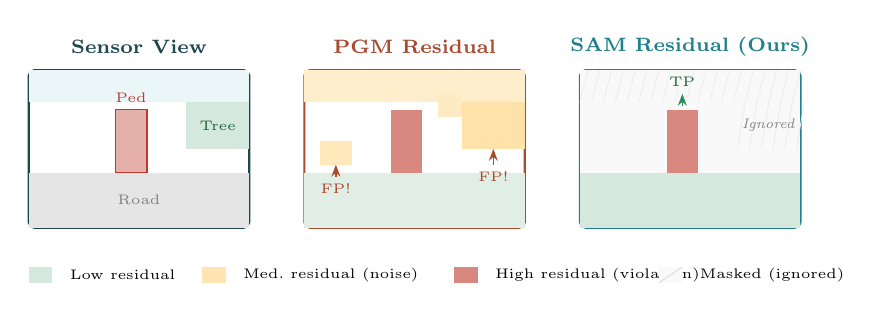
\begin{tikzpicture}[font=\small]

% ---- Column 1: Sensor Input ----
\begin{scope}[shift={(0,0)}]
    % Camera frame placeholder
    \draw[darkteal, line width=0.8pt, rounded corners=2pt] (0,0) rectangle (2.8,2.0);

    % Road surface
    \fill[gray!20] (0,0) rectangle (2.8,0.7);

    % Pedestrian silhouette (small rectangle)
    \fill[dangerzone!40] (1.1,0.7) rectangle (1.5,1.5);
    \draw[dangerzone, line width=0.6pt] (1.1,0.7) rectangle (1.5,1.5);

    % Sky / background
    \fill[lightcyan!30] (0,1.6) rectangle (2.8,2.0);

    % Foliage
    \fill[safezone!20] (2.0,1.0) rectangle (2.8,1.6);

    % Label
    \node[font=\scriptsize\bfseries, text=darkteal] at (1.4,2.3) {Sensor View};
    \node[font=\tiny, text=dangerzone] at (1.3,1.65) {Ped};
    \node[font=\tiny, text=safezone!70!black] at (2.4,1.3) {Tree};
    \node[font=\tiny, text=gray] at (1.4,0.35) {Road};
\end{scope}

% ---- Column 2: PGM Residual (global) ----
\begin{scope}[shift={(3.5,0)}]
    \draw[terracotta, line width=0.8pt, rounded corners=2pt] (0,0) rectangle (2.8,2.0);

    % Global residual heatmap effect
    % Low residual on road
    \fill[safezone!15] (0,0) rectangle (2.8,0.7);

    % High residual on pedestrian
    \fill[dangerzone!60] (1.1,0.7) rectangle (1.5,1.5);

    % Medium residual on foliage (noise!)
    \fill[goldcol!50] (2.0,1.0) rectangle (2.8,1.6);

    % Medium residual on sky boundary
    \fill[goldcol!30] (0,1.6) rectangle (2.8,2.0);

    % Some noise patches
    \fill[goldcol!40] (0.2,0.8) rectangle (0.6,1.1);
    \fill[goldcol!35] (1.7,1.4) rectangle (2.0,1.7);

    % Label
    \node[font=\scriptsize\bfseries, text=terracotta] at (1.4,2.3) {PGM Residual};

    % False positive annotation
    \draw[-{Stealth[length=1.5mm]}, terracotta, line width=0.5pt] (2.4,0.8) -- (2.4,1.0);
    \node[font=\tiny, text=terracotta] at (2.4,0.65) {FP!};

    \draw[-{Stealth[length=1.5mm]}, terracotta, line width=0.5pt] (0.4,0.65) -- (0.4,0.8);
    \node[font=\tiny, text=terracotta] at (0.4,0.5) {FP!};
\end{scope}

% ---- Column 3: SAM Residual (masked) ----
\begin{scope}[shift={(7.0,0)}]
    \draw[tealaccent, line width=0.8pt, rounded corners=2pt] (0,0) rectangle (2.8,2.0);

    % Everything outside mask is suppressed
    \fill[gray!5] (0,0) rectangle (2.8,2.0);

    % Only safety-critical masks are active
    % Pedestrian region: high residual (true positive)
    \fill[dangerzone!60] (1.1,0.7) rectangle (1.5,1.5);

    % Drivable surface: low residual (correct)
    \fill[safezone!20] (0,0) rectangle (2.8,0.7);

    % Ignored regions shown as hatched/faded
    \foreach \x in {0.0,0.15,...,2.8} {
        \draw[gray!15, line width=0.3pt] (\x,1.6) -- (\x+0.1,2.0);
    }
    \foreach \x in {2.0,2.15,...,2.8} {
        \draw[gray!15, line width=0.3pt] (\x,1.0) -- (\x+0.1,1.6);
    }

    % Label
    \node[font=\scriptsize\bfseries, text=tealaccent] at (1.4,2.3) {SAM Residual (Ours)};

    % True positive annotation
    \draw[-{Stealth[length=1.5mm]}, safezone, line width=0.5pt] (1.3,1.55) -- (1.3,1.7);
    \node[font=\tiny, text=safezone!70!black] at (1.3,1.85) {TP};

    % Ignored annotation
    \node[font=\tiny, text=gray] at (2.4,1.3) {\textit{Ignored}};
\end{scope}

% ---- Legend ----
\begin{scope}[shift={(0,-0.7)}]
    \fill[safezone!20] (0,0) rectangle (0.3,0.2);
    \node[font=\tiny, anchor=west] at (0.4,0.1) {Low residual};

    \fill[goldcol!45] (2.2,0) rectangle (2.5,0.2);
    \node[font=\tiny, anchor=west] at (2.6,0.1) {Med.\ residual (noise)};

    \fill[dangerzone!60] (5.4,0) rectangle (5.7,0.2);
    \node[font=\tiny, anchor=west] at (5.8,0.1) {High residual (violation)};

    \fill[gray!5] (8.0,0) rectangle (8.3,0.2);
    \draw[gray!30, line width=0.3pt] (8.0,0) -- (8.3,0.2);
    \node[font=\tiny, anchor=west] at (8.4,0.1) {Masked (ignored)};
\end{scope}

\end{tikzpicture}

    \caption{Qualitative comparison of residual maps. \textbf{Left:} Sensor view showing a pedestrian, road surface, and background foliage. \textbf{Center:} PGM residual---global depth comparison flags foliage and sky boundaries as false positives. \textbf{Right:} SAM residual---semantic masking suppresses background noise while correctly detecting the pedestrian discrepancy.}
    \label{fig:residual_comparison}
\end{figure*}

\subsection{Ablation: Threshold Sensitivity Analysis}

Fig.~\ref{fig:roc_ablation} presents the ROC-style trade-off between TPR and FPR as the residual threshold $\tau$ is swept from $0.1$\,m to $3.0$\,m. \placeholder{Describe the ROC curves. Key insight: PGM requires very high $\tau$ to achieve acceptable FPR, sacrificing TPR. SAM maintains high TPR across all thresholds with consistently low FPR due to semantic masking.}

\begin{figure}[!t]
    \centering
    % ROC-style ablation over residual threshold
% Generated from experiment_results.json
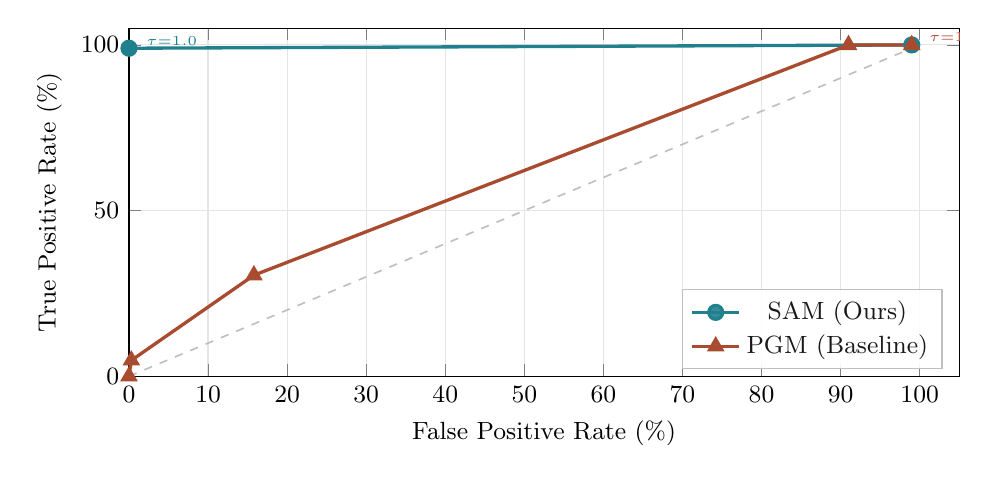
\begin{tikzpicture}
\begin{axis}[
    width=\columnwidth,
    height=6cm,
    xlabel={False Positive Rate (\%)},
    ylabel={True Positive Rate (\%)},
    xmin=0, xmax=105,
    ymin=0, ymax=105,
    grid=major,
    grid style={gray!20},
    legend style={
        at={(0.98,0.02)},
        anchor=south east,
        font=\small,
        draw=gray!50,
        fill=white,
        fill opacity=0.9,
    },
    tick label style={font=\small},
    label style={font=\small},
    every axis plot/.append style={line width=1.2pt, mark size=2.5pt},
]

% SAM (Semantically-Aware Monitor)
\addplot[color=tealaccent, mark=*, mark options={fill=tealaccent}]
    coordinates {
        (0.0, 99.0)    %% tau=1.0
        (99.0, 100.0)    %% tau=0.1
    };
\addlegendentry{SAM (Ours)}

% PGM (Pure Geometric Monitor)
\addplot[color=terracotta, mark=triangle*, mark options={fill=terracotta}]
    coordinates {
        (0.0, 0.0)    %% tau=3.0
        (0.3, 4.8)    %% tau=2.5
        (15.8, 30.5)    %% tau=2.0
        (91.0, 100.0)    %% tau=1.5
        (99.0, 100.0)    %% tau=0.1
    };
\addlegendentry{PGM (Baseline)}

% Diagonal (random classifier)
\addplot[dashed, gray!50, line width=0.6pt, forget plot] coordinates {(0,0) (100,100)};

% Annotations for tau=1.0
\node[font=\tiny, text=tealaccent, anchor=south west] at (axis cs:1.0,97.0) {$\tau{=}1.0$};
\node[font=\tiny, text=terracotta, anchor=south west] at (axis cs:100.0,98.0) {$\tau{=}1.0$};

\end{axis}
\end{tikzpicture}

    \caption{ROC-style ablation over residual threshold $\tau$. The Semantically-Aware Monitor (SAM, \textcolor{tealaccent}{teal}) achieves superior TPR--FPR trade-offs compared to the Pure Geometric Monitor (PGM, \textcolor{terracotta}{terracotta}). \placeholder{Update with experimental data.}}
    \label{fig:roc_ablation}
\end{figure}

\subsection{Response Time Analysis}

Fig.~\ref{fig:response_time} shows the cumulative distribution of safety response times across all trials. \placeholder{Describe the CDF. Key finding: median response time is well below 100ms target for SAM. PGM has similar median but heavier tail due to threshold sensitivity.}

\begin{figure}[!t]
    \centering
    % CDF of Safety Response Times
% Generated from experiment_results.json
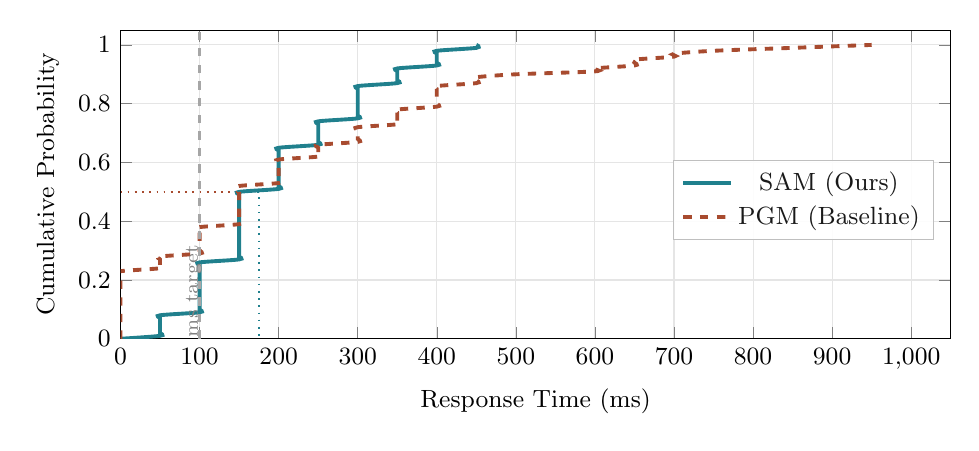
\begin{tikzpicture}
\begin{axis}[
    width=\columnwidth,
    height=5.5cm,
    xlabel={Response Time (ms)},
    ylabel={Cumulative Probability},
    xmin=0, xmax=1050,
    ymin=0, ymax=1.05,
    grid=major,
    grid style={gray!20},
    legend style={
        at={(0.98,0.45)},
        anchor=east,
        font=\small,
        draw=gray!50,
        fill=white,
        fill opacity=0.9,
    },
    tick label style={font=\small},
    label style={font=\small},
    every axis plot/.append style={line width=1.4pt},
    ytick={0, 0.2, 0.4, 0.6, 0.8, 1.0},
]

% SAM CDF
\addplot[color=tealaccent, smooth]
    coordinates {
        (0, 0)
        (50, 0.010)
        (50, 0.020)
        (50, 0.030)
        (50, 0.040)
        (50, 0.050)
        (50, 0.060)
        (50, 0.070)
        (50, 0.080)
        (100, 0.090)
        (100, 0.100)
        (100, 0.110)
        (100, 0.120)
        (100, 0.130)
        (100, 0.140)
        (100, 0.150)
        (100, 0.160)
        (100, 0.170)
        (100, 0.180)
        (100, 0.190)
        (100, 0.200)
        (100, 0.210)
        (100, 0.220)
        (100, 0.230)
        (100, 0.240)
        (100, 0.250)
        (100, 0.260)
        (150, 0.270)
        (150, 0.280)
        (150, 0.290)
        (150, 0.300)
        (150, 0.310)
        (150, 0.320)
        (150, 0.330)
        (150, 0.340)
        (150, 0.350)
        (150, 0.360)
        (150, 0.370)
        (150, 0.380)
        (150, 0.390)
        (150, 0.400)
        (150, 0.410)
        (150, 0.420)
        (150, 0.430)
        (150, 0.440)
        (150, 0.450)
        (150, 0.460)
        (150, 0.470)
        (150, 0.480)
        (150, 0.490)
        (150, 0.500)
        (200, 0.510)
        (200, 0.520)
        (200, 0.530)
        (200, 0.540)
        (200, 0.550)
        (200, 0.560)
        (200, 0.570)
        (200, 0.580)
        (200, 0.590)
        (200, 0.600)
        (200, 0.610)
        (200, 0.620)
        (200, 0.630)
        (200, 0.640)
        (200, 0.650)
        (250, 0.660)
        (250, 0.670)
        (250, 0.680)
        (250, 0.690)
        (250, 0.700)
        (250, 0.710)
        (250, 0.720)
        (250, 0.730)
        (250, 0.740)
        (300, 0.750)
        (300, 0.760)
        (300, 0.770)
        (300, 0.780)
        (300, 0.790)
        (300, 0.800)
        (300, 0.810)
        (300, 0.820)
        (300, 0.830)
        (300, 0.840)
        (300, 0.850)
        (300, 0.860)
        (350, 0.870)
        (350, 0.880)
        (350, 0.890)
        (350, 0.900)
        (350, 0.910)
        (350, 0.920)
        (400, 0.930)
        (400, 0.940)
        (400, 0.950)
        (400, 0.960)
        (400, 0.970)
        (400, 0.980)
        (450, 0.990)
        (450, 1.000)
    };
\addlegendentry{SAM (Ours)}

% PGM CDF
\addplot[color=terracotta, smooth, dashed]
    coordinates {
        (0, 0)
        (0, 0.010)
        (0, 0.020)
        (0, 0.030)
        (0, 0.040)
        (0, 0.050)
        (0, 0.060)
        (0, 0.070)
        (0, 0.080)
        (0, 0.090)
        (0, 0.100)
        (0, 0.110)
        (0, 0.120)
        (0, 0.130)
        (0, 0.140)
        (0, 0.150)
        (0, 0.160)
        (0, 0.170)
        (0, 0.180)
        (0, 0.190)
        (0, 0.200)
        (0, 0.210)
        (0, 0.220)
        (0, 0.230)
        (50, 0.240)
        (50, 0.250)
        (50, 0.260)
        (50, 0.270)
        (50, 0.280)
        (100, 0.290)
        (100, 0.300)
        (100, 0.310)
        (100, 0.320)
        (100, 0.330)
        (100, 0.340)
        (100, 0.350)
        (100, 0.360)
        (100, 0.370)
        (100, 0.380)
        (150, 0.390)
        (150, 0.400)
        (150, 0.410)
        (150, 0.420)
        (150, 0.430)
        (150, 0.440)
        (150, 0.450)
        (150, 0.460)
        (150, 0.470)
        (150, 0.480)
        (150, 0.490)
        (150, 0.500)
        (150, 0.510)
        (150, 0.520)
        (200, 0.530)
        (200, 0.540)
        (200, 0.550)
        (200, 0.560)
        (200, 0.570)
        (200, 0.580)
        (200, 0.590)
        (200, 0.600)
        (200, 0.610)
        (250, 0.620)
        (250, 0.630)
        (250, 0.640)
        (250, 0.650)
        (250, 0.660)
        (300, 0.670)
        (300, 0.680)
        (300, 0.690)
        (300, 0.700)
        (300, 0.710)
        (300, 0.720)
        (350, 0.730)
        (350, 0.740)
        (350, 0.750)
        (350, 0.760)
        (350, 0.770)
        (350, 0.780)
        (400, 0.790)
        (400, 0.800)
        (400, 0.810)
        (400, 0.820)
        (400, 0.830)
        (400, 0.840)
        (400, 0.850)
        (400, 0.860)
        (450, 0.870)
        (450, 0.880)
        (450, 0.890)
        (500, 0.900)
        (600, 0.910)
        (600, 0.920)
        (650, 0.930)
        (650, 0.940)
        (650, 0.950)
        (700, 0.960)
        (700, 0.970)
        (750, 0.980)
        (850, 0.990)
        (950, 1.000)
    };
\addlegendentry{PGM (Baseline)}

% 100ms target line
\draw[dashed, gray!70, line width=0.8pt] (axis cs:100,0) -- (axis cs:100,1.05);
\node[font=\scriptsize, text=gray, rotate=90, anchor=south] at (axis cs:115,0.10) {100\,ms target};

% Median annotations
\draw[dotted, tealaccent, line width=0.6pt] (axis cs:0,0.5) -- (axis cs:175,0.5) -- (axis cs:175,0);
\node[font=\tiny, text=tealaccent] at (axis cs:175,-0.08) {175};
\draw[dotted, terracotta, line width=0.6pt] (axis cs:0,0.5) -- (axis cs:150,0.5);
\node[font=\tiny, text=terracotta] at (axis cs:158,-0.08) {150};

\end{axis}
\end{tikzpicture}

    \caption{Cumulative distribution of safety response times. The vertical dashed line marks the 100\,ms target. \placeholder{Update with experimental data.}}
    \label{fig:response_time}
\end{figure}

% ============================================================
% VII. DISCUSSION
% ============================================================
\section{Discussion}
\label{sec:discussion}

\subsection{Semantic Filtering as a Prerequisite for Robust Monitoring}

Our ablation study confirms the central hypothesis: a pure geometric monitor suffers from an unacceptably high false positive rate in realistic environments. Depth residuals arise naturally from benign sources---foliage sway, specular reflections, sky-boundary artifacts, and minor misalignments between the neural render and sensor frame. The PGM treats all such residuals equally, leading to frequent false alarms that would make the system impractical for deployment.

The semantically-aware monitor eliminates this issue by restricting residual computation to pixels belonging to safety-critical classes. Background noise in sky, vegetation, and building facades is ignored entirely, focusing the monitor's attention on what matters: dynamic actors in the vehicle's path and the integrity of drivable surfaces.

\subsection{Limitations}

Several limitations of our current approach warrant discussion:

\begin{itemize}
    \item \textbf{Perfect localization assumption:} We rely on ground-truth poses from CARLA. In practice, pose estimation errors from visual-inertial odometry or LiDAR-inertial odometry would introduce additional residuals that the monitor must distinguish from genuine map failures.
    \item \textbf{Semantic oracle:} Our ground-truth semantic segmentation from CARLA represents an idealized sensor. A deployed system would require a learned semantic segmentation model, introducing its own error characteristics.
    \item \textbf{Binary intervention:} The current baseline controller implements full emergency braking. A more sophisticated approach could employ graduated responses (e.g., speed reduction, lane change) based on the severity and spatial location of the detected violation.
    \item \textbf{Single-agent evaluation:} We evaluate in a controlled single-agent scenario. Multi-agent interactions and complex traffic scenarios remain future work.
\end{itemize}

\subsection{Connection to Course Themes}

This work directly connects to the validation of safety-critical systems (AA228V/CS238V). The Simplex Architecture provides a principled framework for using unverified components (the 3DGS map) while maintaining safety guarantees through runtime monitoring. Our safety specification $\phi_{\text{safe}}$ formalizes the properties that the neural map must satisfy, and our monitor implements a decision procedure for checking these properties at runtime. The ablation study demonstrates the importance of the monitoring strategy: a naively specified monitor (PGM) can achieve high sensitivity but at the cost of excessive false alarms, while a carefully designed monitor (SAM) achieves both high sensitivity and high specificity.

% ============================================================
% VIII. CONCLUSION
% ============================================================
\section{Conclusion}
\label{sec:conclusion}

We presented \textsc{Simplex-Splat}, a runtime verification framework that bridges the trust gap between neural 3DGS maps and safety-critical autonomous navigation. By adapting the Simplex Architecture from the control domain to the perception domain, we demonstrated that a semantically-aware residual monitor can reliably detect neural map failures---including unmodeled dynamic actors and unconverged static geometry---while maintaining a false positive rate compatible with practical deployment.

Our ablation study quantified the critical importance of semantic filtering: a pure geometric monitor achieves high detection rates but produces frequent false alarms in unstructured environments, while our semantically-aware variant restricts attention to safety-critical classes, achieving robust verification without excessive conservatism. \placeholder{Summarize key numerical results once available.}

Future work includes relaxing the perfect localization assumption via integration with robust state estimation, replacing the semantic oracle with a learned segmentation model with calibrated uncertainty, and extending the framework to multi-agent scenarios with inter-vehicle communication.

% ============================================================
% CONTRIBUTIONS
% ============================================================
\section*{Contributions}

\textbf{Rahul Ayanampudi:} CARLA simulation integration, SplaTAM pipeline modification and online 3DGS map management, scenario design (pedestrian spawning, obstacle placement), data collection for experimental evaluation.

\textbf{Carlo Schreiber:} Safety specification formalization ($\phi_{\text{safe}}$), semantically-aware residual monitor design and implementation, Simplex Architecture integration, ablation study design, primary paper writing and figure generation.

% ============================================================
% REFERENCES
% ============================================================
\printbibliography

\end{document}
